\documentclass{standalone}
\usepackage{standalone}

\begin{document}
\chapter{Methodology}
\label{chap:method}
After reviewing all the previous works in Bengali POS tagging, we have noticed some properties in these methods
\begin{itemize}
    \item  From the comparison by Mukherjee and Mandal\cite{mukherjee}, we see that all the models show an average accuracy of 85\%-90\% on their dataset but in case of the NLTK dataset, they show at best 82\%. 
    \item Most of the models use other models or tools like NER, stemmer, lexicon development. So the performance of these models depends on the performance of these tools or models. 
    \item Most of the models either use probabilistic methods or use other features for training the neural networks. Neither of them uses probability as features for the network.

\end{itemize}
From these points, we had some primary goals to fulfill -
\begin{itemize}
    \item use probability as an feature for training the network. 
    \item Reduce dependency on other tools
    \item check all possible set of tag to get the best tagset
\end{itemize}
Most of the models either use probabilistic methods or use other features for training the neural networks. Neither of them uses probability as features for the network. So we started with a new model based on the model proposed by Uddin, Khan, Islam, and Jannat\cite{uddin}.In the model, we will use the words’ respected probability as the feature for the neural network We also proposed to use the Prefix Tree (trie) and Dynamic Programming approach to reduce time and space complexity.
\section{Probability as Feature}
\label{feature}
In English POS Tagging, different features have been used like :
\begin{itemize}
    \item If the word starts with a capital letter
    \item If the word contains digits or hyphen
    \item Suffixes and prefixes of the word
    \item Complete capitalized word
\end{itemize}
In Bengali, there is nothing like the capital letter. It is also hard to find the suffix and prefix of the word in Bengali. So we have decided to use the probability of their perspective tag as feature.
\subsection{Probability Calculation}
At first, we have calculated the frequency of all our words being each POS. Then we  have got the probabilities in the method described below :
\begin{itemize}
    \item Equation to calculate probability
    \begin{equation}\label{eq1}
    P(x,a) = \frac{cnt(x,a)}{cntAll(x)}
    \end{equation}
 \begin{displaymath} P(x, a) = the\:probability\:of \:word\:x\:being\:the\:POS\:a,\end{displaymath}
  \begin{displaymath}
   cnt(x, a) = the\:total\:number\:count\:of\:word\:x\:being\:POS\:a
  \end{displaymath}
   \begin{displaymath}
   cntAll(x) = the\:total\:occurrence\:of\:the\:word\:x\:in\:the\:dataset
  \end{displaymath}
  \end{itemize}
  \subsection{Feature Calculation}
   For every word and tag, the probability feature will be calculated as :
  \begin{itemize}
  \item the input features will be :
  \begin{itemize}
        \item {\bf Adjective}       : 0 + P(x, Adjective)
        \item {\bf Adverb}          : 1 + P(x, Adverb)
        \item {\bf Conjunction}     : 2 + P(x, Conjunction)
        \item {\bf Demonstrative}   : 3 + P(x, Demonstrative)
        \item {\bf Noun}            : 4 + P(x, Noun)
        \item {\bf Particle}        : 5 + P(x, Particle)
        \item {\bf Postposition}    : 6 + P(x, Postposition)
        \item {\bf Pronoun}         : 7 + P(x, Pronoun)
        \item {\bf Punctuation}     : 8 + P(x, Punctuation)
        \item {\bf Quantifier}      : 9 + P(x, Quantifier)
        \item {\bf Residuals}       : 10 + P(x, Residuals)
        \item {\bf Verb}            : 11 + P(x, Verb)
  \end{itemize}
 
\item The output feature will be :
\begin{itemize}
        \item {\bf Adjective}       : 0 
        \item {\bf Adverb}          : 1 
        \item {\bf Conjunction}     : 2 
        \item {\bf Demonstrative}   : 3 
        \item {\bf Noun}            : 4 
        \item {\bf Particle}        : 5 
        \item {\bf Postposition}    : 6 
        \item {\bf Pronoun}         : 7 
        \item {\bf Punctuation}     : 8 
        \item {\bf Quantifier}      : 9 
        \item {\bf Residuals}       : 10 
        \item {\bf Verb}            : 11 
  \end{itemize}
\end{itemize}
\section {Prefix Tree (Trie)}]
Trie,also known as the prefix tree is a kind of search tree data structure that stores data especially strings in a structured way. It was first introduced by Rene de la Briandais in 1959\cite{de1959file}\cite{trie}.The term trie was coined two years later by Edward Fredkin\cite{black1998dictionary}\cite{trie}. The term was found from the word retrieve\cite{trie}.It's searching technique mainly based on the matched prefix of the words.\\
\begin{figure}[h!]
\centering
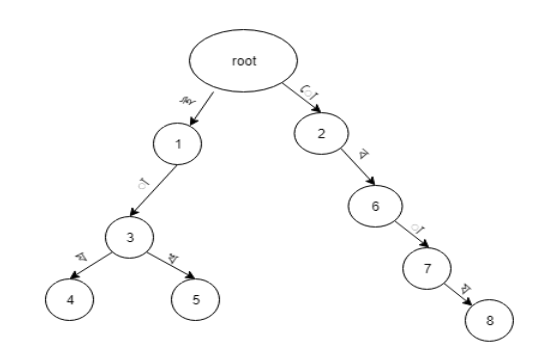
\includegraphics[width=1.0\columnwidth]{img/trie.png}
\caption{Trie Structure}
\label{trie}
\end{figure}
We have used Trie Data Structure in both Data Preprocessing stem to calculate the frequency and during both the train and the evaluation process. Without Trie, the searching process would take a lot more time complexity. For each word search, it can be O(N), where N is the summation of all the words’ length in the dictionary without trie. Using trie it would be only O(n), where n is the length of the searched word. We have stored all the words in the dataset as a string and their frequencies in the leaf nodes. 
\section{Training Process}
\label{train}
According to the model proposed in the paper\cite{uddin}, The Neural Network will have a simple structure of 3 layers containing 5,3 and 1 nodes. First layer of 5 nodes will receive the word’s, it’s previous two words’ and the next two words’ probability feature as input. And the last layer will provide the output
\begin{figure}[h!]
\centering
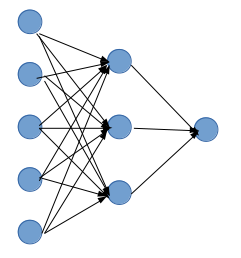
\includegraphics[width=1.0\columnwidth]{img/Network.png}
\caption{Neural Network Structure}
\label{neural}
\end{figure}
But We have decided to uexperiment with more network architectures for training purposes like Sequential Model, Bi-Directional LSTM.
\section{Tagging Process}
\label{tagging}
One of the most important parts of our research was the tagging process. We would generate all possible sets of tags. For a set, we would calculate the error score by matching it to the networks predicted result. So for each word, we would give the network the probabilistic feature input of the word’s, it’s previous two words, and the next two words. If they are absent we would provide 0 as input. If the predicted result does not match the generated result we add  1 to the error score. The set with the minimum error score is our result tag set.
\subsection{Complexity Analysis}
As we are generating all sets or combinations of tags of a line then this will generate all 12$^n$ combinations. That means it will have the time complexity of O(12$^n$). Which is in case of lines having more than 8 words is a huge time complexity to bear for a single line. So we have introduced the Dynamic Programming method to resolve this issue.
\subsection{Dynamic Programming Method}
Here we can divide the problem into subproblems. As we are giving only the five consecutive words’ features as input while generating the best answer we only need to care about these five consecutive tags. So  we can compute the best result as the DP function :\\
   DP[tag1][tag2][tag3][tag4][pos] = MAX(DP[tag2][tag3][tag4][1][pos+1]+ score(tag1,tag2,tag3,tag4,1),DP[tag2][tag3][tag4][2][pos+1]+score(tag1,tag2,tag3,tag4,2), . . . . . , DP[tag2][tag3][tag4][12][pos+1]+score(tag1,tag2,tag3,tag4,12)) 
   \begin{itemize}
       \item tag1 is the tag of word[pos-2]
        \item tag2 is the tag of word[pos-1]
         \item tag3 is the tag of word[pos]
          \item tag4 is the tag of word[pos+1]
          \item score(tag1,tag2,tag3,tag4,i) = 1 if predicted tag for input set tag1,tag2,tag3,tag4 and i is tag3 otherwise 0.
   \end{itemize}
This has reduced our complexity to O(12$^5$) for each word. That is O(12$^5$*n) for each line where n is the number of words in a line which is a huge improvement comparing to the O(12$^n$) 
\subsection{Unknown Words}
While tagging there is a huge chance of countering some unknown words. To sort that out, we have decided to use the XML dictionary. We will consider the word will have the most probability of 0.78 of being the tag in the dictionary. And other tags will have a probability sharing of 0.02%.

\end{document}